\chapter{Optimizing Calls and Object Model}
\label{chp:ch5-object}

Being a object oriented programing language, it is a common practice for Python programmer to encode states using classes and encapsulate logic in methods in their programs.
It is essential for us to ensure the performance of object operations and method calls in ZipPy.
In the previous chapters we discussed how we optimize arithmetics (Chapter~\ref{chp:ch3-zippy}) and accelerate iterators (Chapter~\ref{chp:ch4-peeling}),
in this chapter we explain how we structure call sites and object operations in ZipPy.

\section{Call Site Modeling}

Calls are common in Python programs.
In general you can call any \emph{callable} object in Python.
Making a call in different contexts has different semantics allowing the caller to pass arguments to the callee in different ways.

\subsection{The Structure of Call Sites in Python}

\begin{figure}
\centering
\subfigure[Simple call site]{
	
\includegraphics[scale=.9]{figures/ch5-call-site-simple-code}
	\label{fig:ch5-call-site-simple-code}
}
\subfigure[Attribute call site]{
	
\includegraphics[scale=.9]{figures/ch5-call-site-attribute-code}
	\label{fig:ch5-call-site-attribute-code}
}
\caption{Basic syntax of calls in Python}
\label{fig:ch4-call-site-synteax-code}
\end{figure}

Figure~\ref{fig:ch5-call-site-simple-code} shows the syntax of a simple call in Python.
It is simple enough for us to explain the basic steps of making a call in Python without getting into more complicated details.
The execution of the call shown in the Figure involves the following steps.
As the first step, the program needs to look up the symbol \texttt{foo} from the current scope or its enclosing scope with respect to Python's scoping rules.
After resolving the symbol \texttt{foo}, the program then checks the type of the resolved object to determine the eligibility of such call.
Lastly, the actual call takes place using a calling convention that matches the type of the callee object.
The Python interpreter uses different calling convention or passes the arguments to the callee in a different way depending on the actual type of the callee.
For instance, if the callee is a Python class object, the interpreter creates an empty Python object and passes it to the callee as the first argument.

The call site shown in Figure~\ref{fig:ch5-call-site-simple-code} is in its simplest form.
We refer it as a \emph{simple call site}.
The callee resolution for the call shown in Figure~\ref{fig:ch5-call-site-attribute-code} involves an attribute referencing on the Python object \texttt{p}.
We refer this type of call sites as \emph{attribute call sites}, since the actual callee is an attribute of the primary object like \texttt{p} in the Figure.
The primary object, however, can be any namespace backed by a Python object such as a regular object, a class object or a module.
Looking back at the simple call site as shown in Figure~\ref{fig:ch5-call-site-simple-code},
it is worth noting that the callee resolution might involve an attributing referencing as well depending on the type of the scope in which the call takes place.
For example, if program resolves \texttt{foo} as a global variable, the look up of \texttt{foo} includes an implicit attribute referencing on the current Python module.
Similarly, in a class scope, a simple call to an existing class attribute also involves an implicit attribute look up on the enclosing class object.
% say something about motivates the structure of the AST
The same syntax implies different semantics and ways to make the actual call at runtime.
To capture this variation, we decompose a call site in Python into multiple components and assemble them in different ways to serve different variations.
This way allows us to apply specializations on each component separately to accelerate calls in Python programs.

\subsubsection{The AST of Call Sites}

\begin{figure}
\centering
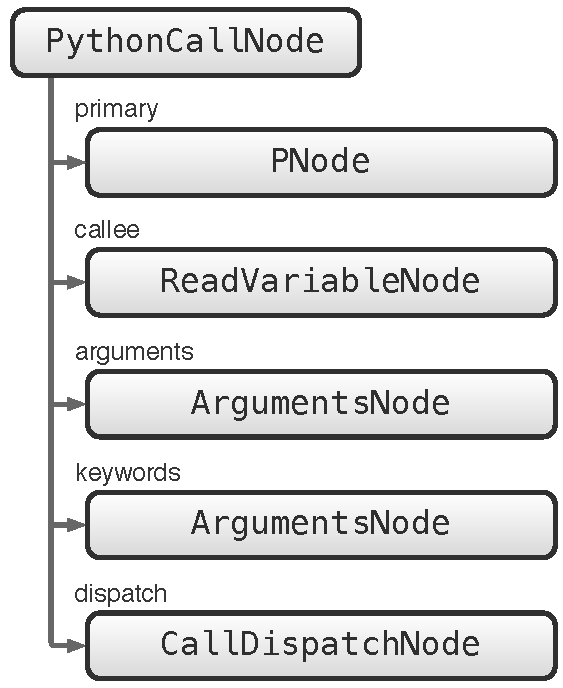
\includegraphics[scale=.5]{figures/ch5-python-call-node-basic}
\caption{The structure of a \texttt{PythonCallNode}}
\label{fig:ch5-python-call-node-basic}
\end{figure}

Figure~\ref{fig:ch5-python-call-node-basic} illustrates the basic structure of a call node in ZipPy.
A \texttt{PythonCallNode} employees five child nodes representing five components of the call site.
Each child node can further expand into its own sub tree depending on the complexity of the component.
A call node performs a Python call in-coorperating its child nodes in the following steps:

\begin{enumerate}

\item The primary node evaluates the primary object of the call.
If the primary component is missing, the primary node returns the constant Python \texttt{None} object.

\item The callee node resolves the actual callee object using the previously resolved primary object if necessary.
If the callee resolution does not involve an attribute referencing, it ignores the primary object.

\item The arguments node evaluates all the arguments, and returns them to the call node as a Java array.

\item The keywords node evaluates all the keyword arguments, and returns them to the call node in an Java array.

\item The \texttt{PythonCallNode} passes the evaluated primary object, callee, arguments array and keyword arguments array to the dispatch node.
The dispatch node performs the actual call using inline caching based dispatch chain scheme~\ref{?}, which we will explain in more in detail in Section~\ref{?}.

\end{enumerate}

\section{Object Model}
